%% MQ-06-effects.tex
\chapter{Effects}

Mystic Quest uses a quite elaborate system of effects and stats. Most of them are represented with icons in-game. A shame that they were not documented at all.

\begin{longtable}{ l l p{7cm} }
	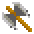
\includegraphics[height=1em,keepaspectratio]{./resources/effects/axe}
	& Axes 
	& Weapon type
\\ \hline
	
\includegraphics[height=1em,keepaspectratio]{./resources/effects/blind}
	& Blind 
	& Lowers accuracy of target.
\\ \hline
	
\includegraphics[height=1em,keepaspectratio]{./resources/effects/bomb}
	& Bombs 
	& Weapon type
\\ \hline
	
\includegraphics[height=1em,keepaspectratio]{./resources/effects/confusion}
	& Confuse 
	& Affected party members do target at random, incl. other party members
\\ \hline
	
\includegraphics[height=1em,keepaspectratio]{./resources/effects/drain}
	& Drain 
	& Usually lowers stats. Sometimes refills stats of caster.
\\ \hline
	
\includegraphics[height=1em,keepaspectratio]{./resources/effects/damage}
	& Physical 
	& Damage type.
\\ \hline
	
\includegraphics[height=1em,keepaspectratio]{./resources/effects/earth}
	& Earth 
	& Damage type.
\\ \hline
	
\includegraphics[height=1em,keepaspectratio]{./resources/effects/fatal}
	& Fatal
	& Spell effect. When cast successfully the target is put into fatal condition. \nameref{spell:life} counters the effect.
\\ \hline
	
\includegraphics[height=1em,keepaspectratio]{./resources/effects/fire}
	& Fire 
	& Damage type.
\\ \hline
	
\includegraphics[height=1em,keepaspectratio]{./resources/effects/paralyze}
	& Paralyze 
	& Target skips turns until effect wears off
\\ \hline
	
\includegraphics[height=1em,keepaspectratio]{./resources/effects/petrify}
	& Petrify 
	& Target is turned into stone and skips turns. Effect does not wear off over time.
\\ \hline
	
\includegraphics[height=1em,keepaspectratio]{./resources/effects/poison}
	& Poison 
	& Target takes additional damage every turn
\\ \hline
	
\includegraphics[height=1em,keepaspectratio]{./resources/effects/shoot}
	& Shoot 
	& Weapon type
\\ \hline
	
\includegraphics[height=1em,keepaspectratio]{./resources/effects/silence}
	& Silence 
	& Target cannot cast spells
\\ \hline
	
\includegraphics[height=1em,keepaspectratio]{./resources/effects/sleep}
	& Sleep 
	& Target skips turns until effect wears off
\\ \hline
	
\includegraphics[height=1em,keepaspectratio]{./resources/effects/water}
	& Water 
	& Damage type
\\ \hline
	
\includegraphics[height=1em,keepaspectratio]{./resources/effects/wind}
	& Wind 
	& Damage type
\end{longtable}

There is a little problem with the effects granted by armor and weapon to the companion: If you first load a late game savegame with a companion well equipped, and then start a new game, the effects of the savegame are not cleared. And your companions are much more beefy than they are supposed to be.

This bug coined the phrase: As soon as you load a game, you're cheating.
